\documentclass[10pt,a4paper]{article}
\usepackage[latin1]{inputenc}
\usepackage{amsmath}
\usepackage{microtype}
\usepackage[none]{hyphenat}
\usepackage{verbatim}
\usepackage{amsfonts}
\usepackage{amssymb}
\usepackage{enumitem}
\renewcommand{\familydefault}{\sfdefault}
\usepackage{mathpazo}
\renewcommand{\rmdefault}{put}
\usepackage{enumitem}
\usepackage[dvipsnames,svgnames]{xcolor}
\usepackage{tkz-euclide}
\usetkzobj{all}
\usepackage{graphicx}
\usepackage{tikz} 	
\usepackage{adjustbox}
\usepackage{multicol}
\usepackage{lipsum}
\usepackage[left=0.1cm,right=0.7cm,top=0.2cm,bottom=1.5cm]{geometry}
\usepackage{cancel} \usepackage{xcolor}
\usepackage{tcolorbox}
\usetikzlibrary{decorations.pathmorphing,patterns}
\usetikzlibrary{decorations.pathreplacing,calc}
 \newcommand\coret[2][red]{\renewcommand\CancelColor{\color{#1}}\cancel{#2}}
\SetLabelAlign{Center}{\hfil\makebox[1.0em]{#1}\hfil}

%%_------= solusi


% Set this =0 to hide, =1 to show

% Set this =0 to hide, =1 to show
\newtcolorbox{mybox}[1][] { colframe = blue!10, colback = blue!3,boxsep=0pt,left=0.2em, coltitle = blue!20!black, title = \textbf{jawab}, #1, } 

%---------- kunci (jika 1 ) muncul
\def\tampilkunci{1}
\newcommand{\hide}[1]{\ifnum\tampilkunci=1
%
\begin{mybox}
 #1
\end{mybox}
%
\vspace{\baselineskip}\fi}



\newcommand*\cicled[1]{\tikz[baseline=(char.base)]{\node[white, shape=circle, fill=red!80,draw,inner sep=0.5pt](char){#1};}}

\newcommand*\kunci[1]{\ifnum\tampilkunci=1
%
\tikz[baseline=(char.base)]{\node[red, shape=circle,draw,inner sep=0.5pt,xshift=2pt](char){#1};}\stepcounter{enumii}
\fi\ifnum\tampilkunci=0
%
\hspace{3pt}#1\stepcounter{enumii}
%
\fi}

\newcommand*\silang[1]{\tikz[baseline=(char.base)]{
\draw[red,thick](-0.2,-0.20)--(0.2,0.2);
\draw[red,thick](-0.2,0.20)--(0.2,-0.2);
\node[black](char){#1};
}}

\newcommand*\centang[1]{\tikz[baseline=(char.base)]{
\draw[red, very thick](-0.2,0.1)--(-0.1,0)--(0.2,0.3);
\node(char){#1};
}}

\newcommand*\merah[1]{
\textcolor{red}{#1}}
\newcommand*\pilgan[1]{
\begin{enumerate}[label=\Alph*., itemsep=0pt,topsep=0pt,leftmargin=*,align=Center] #1 
\end{enumerate}}
\newcommand*\pernyataan[1]{
\begin{enumerate}[label=(\arabic*), itemsep=0pt,topsep=0pt,leftmargin=*] #1 
\end{enumerate}}

\begin{document}

\setlength{\abovedisplayskip}{0pt}
\setlength{\belowdisplayskip}{3pt}
\setlength{\abovedisplayshortskip}{0pt}
\setlength{\belowdisplayshortskip}{3pt}
%-----------------------------------------------

 \centering
  \renewcommand{\arraystretch}{2}
  \begin{tabular}{  |>{\centering\arraybackslash}m{4cm}|%
                    >{\centering\arraybackslash}m{11cm}|%
                    >{\centering\arraybackslash}m{4cm}|%
  }
    \hline
    \vspace{0.15cm} 
    \tikz[baseline=(char.base)]{
\draw[green!80!black](-0.3,-0.2) rectangle (0.3,0.2);
\node[green](char){line};
} \small{ arifstwan} &       \textbf{Soal Modul Termodinamika } 
          &  bintangpelajar.com
  \\ \hline 
    
  \end{tabular}
\setlength{\columnsep}{0pt}
\vspace{0.15cm}

\begin{multicols*} {3} 
\newcommand{\tikzmark}[2]{\tikz[remember picture,baseline=(#1.base)]{\node[inner sep=0pt] (#1) {#2};}} 


\begin{enumerate}[itemsep=0mm]

%------------ nomor 1----------
\item Perhatika grafik hubungan tekanan $(p)$ terhadap volume $(V)$ gas berikut ini.

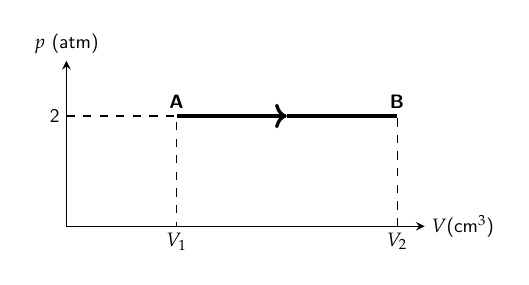
\begin{tikzpicture}[scale=0.7]
\draw[stealth-stealth](0,3)node[above,scale=0.7]{$p$ (atm)}--(0,0)--(6.5,0)node[right,scale=0.7]{$V$(cm$^3$)};
\draw[very thick,->](2,2)node [above,scale=0.7]{\textbf{A}}--(4,2);
\draw[very thick](4,2)--(6,2)node [above,scale=0.7]{\textbf{B}};
\draw[dashed](0,2)--(2,2)--(2,0);
\node at (0,2) [left,scale=0.7]{2};
\node at (2,0) [below,scale=0.7]{$V_1$};
\node at (6,0) [below,scale=0.7]{$V_2$};
\draw [dashed](6,0)--(6,2);
\end{tikzpicture}

Jika $V_1$ = 100 cm$^3$ dan $V_2$ = 300 cm$^3$ usaha yang dilakukan gas dari keadaan (A) ke keadaan (B) adalah . . . .
\pilgan{
\item 20 J
\item [\kunci{B.}] 40 J
\item 80 J
\item 200 J
\item 400 J
}
\hide{
\small{\begin{align*}
W &= p.\Delta V\\
W &= 2 (\text{atm}).(300(\text{cm}^3)-100(\text{cm}^3))\\
W &= 2 \times 10^5 (300\times 10^{-6}-100\times 10^{-6})\\
W &= 2 \times 10^5(200\times 106{-6})\\
W &= 40J
\end{align*}}
} 

%--------------- nomor 2 -----------
\item Suatu gas yang volumenya 0,5 m$^3$ perlahan-lahan dipanaskan dengan tekanan tetap hingga volumenya 2 m$^3$. Jika usaha luar adalah 3 $\times 10^5$ J, maka tekanan gas tersebut adalah . . .
\pilgan{
\item 1,5 $\times 10^5$ N/m$^2$
\item [\kunci{B.}] 2,0 $\times 10^5$ N/m$^2$
\item 3,0 $\times 10^5$ N/m$^2$
\item 4,0 $\times 10^5$ N/m$^2$
\item 5,0 $\times 10^5$ N/m$^2$
}
\hide{
rumus usaha pada termodinamika (tekanan tetp)
\begin{align*}
W&=p.\Delta V\\
3 \times 10^5&= p.(2-0.5)\\
p&= \frac{3\times 10^5}{1.5}\\
p&=2\times 10^5 \text{Pa}
\end{align*}
}

%------------------- nomor 3 ----------
\item Satu mol gas ideal yang menempati suatu silinder berpengisap tanpa gesekan, mula-mula suhu gas adalah $T$. Kemudian, gas tersebut dipanaskan pada tekanan konstan sehingga volumenya menjadi 4 kali lebih besar. Jika $R$ adalah tetapan gas universal, bersarnya usaha yang telah dilakukan oleh gas untuk menaikkan volumenya tersebut adalah . . . 
\pilgan{
\item $\frac{RT}{4}$
\item $RT \ln 4$
\item $6 RT $
\item $4 RT$
\item [\kunci{E.}]$3 RT$
}
\hide{
\begin {align*}
W&=p.\Delta V = p(V_2-V_1)\\
W&=p.(4V-V)\\
W&=p.3V
\end{align*}
Kemudian disubtitusikan dengan persamaan umum gas
\begin{align*}
pV&=nRT\\
w&=3pV\\
w&=3.nRT\\
w&=3RT
\end{align*}}

% ------------ nomor 4 ------------
\item Usaha yang dilakukan oleh gas ideal yang mengalami proses isokhorik dari tekanan $p_1$ hingga $p_2$ adalah . . . .
\pilgan{
\item [\kunci{A.}]0
\item $p_1.V_2$
\item $p_2.V_2$
\item $\frac{p_1+p_2}{2}\times \frac{V_1+V_2}{2}$
\item $(p_1-p_2)V$
}
\hide{
Pada proses isokhorik usaha gas ideal pada perubahan volume nol (volume tetap)
$$W=p.\Delta V=p.0=0$$ Tidak ada perubahan volume, maka usahanya nol.
 }

%----------------- nomor 5 ------
\item Suatu gas ideal mengalami proses siklus seperti diagram $p-V$ berikut.

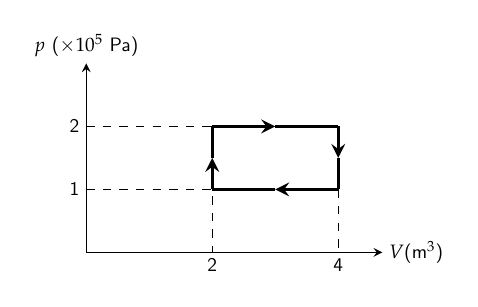
\begin{tikzpicture}[scale=0.8]
\draw[stealth-stealth](0,3)node[above,scale=0.7]{$p$ ($\times 10^5$ Pa)}--(0,0)--(4.7,0)node[right,scale=0.7]{$V$(m$^3$)};
\draw[very thick,-stealth](2,2)--(3,2);
\draw [very thick,-stealth](4,2)--(4,1.5);
\draw [very thick,-stealth](4,1)--(3,1);
\draw [very thick,-stealth](2,1)--(2,1.5);
\draw [very thick](3,2)--(4,2)(4,1.5)--(4,1)(3,1)--(2,1)(2,1.5)--(2,2);;
\draw[dashed](0,2)--(2,2)(0,1)--(2,1)--(2,0)(4,1)--(4,0);
\node at (0,2) [left,scale=0.7]{2};
\node at (0,1) [left,scale=0.7]{1};
\node at (2,0) [below,scale=0.7]{2};
\node at (4,0) [below, scale =0.7]{4};
\end{tikzpicture}



Usaha yang dihasilkan pada siklus ini adalah. . . .
\pilgan{
\item [\kunci{A.}]200 kJ
\item 400 kJ
\item 600 kJ
\item 800 kJ
\item 1.000 kJ
}
\hide{
Besarnya usaha pada suatu siklus adalah luas grafik

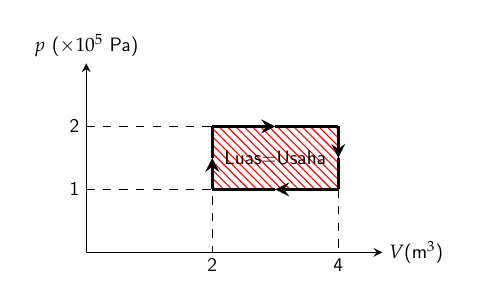
\begin{tikzpicture}[scale=0.8]
\draw[stealth-stealth](0,3)node[above,scale=0.7]{$p$ ($\times 10^5$ Pa)}--(0,0)--(4.7,0)node[right,scale=0.7]{$V$(m$^3$)};
\draw [pattern=north west lines, pattern color=red](2,1) rectangle (4,2);
\draw[very thick,-stealth](2,2)--(3,2);
\draw [very thick,-stealth](4,2)--(4,1.5);
\draw [very thick,-stealth](4,1)--(3,1);
\draw [very thick,-stealth](2,1)--(2,1.5);
\draw [very thick](3,2)--(4,2)(4,1.5)--(4,1)(3,1)--(2,1)(2,1.5)--(2,2);;
\draw[dashed](0,2)--(2,2)(0,1)--(2,1)--(2,0)(4,1)--(4,0);
\node at (0,2) [left,scale=0.7]{2};
\node at (0,1) [left,scale=0.7]{1};
\node at (2,0) [below,scale=0.7]{2};
\node at (4,0) [below, scale =0.7]{4};
\node at (3,1.5)[scale=0.7]{Luas=Usaha};
\end{tikzpicture}
\begin{align*}
W&=(V_2-V_1)(p_2-p_1) \\
W&=(4-2)(2-1)\times 10^5\\
W&=200 \text{ kJ}
\end{align*}
} 

%-------------- nomor 6  ---------
\item Suatu mesin kalor bekerja dengan siklus yang dibangun dari dua proses isobar dan dua proses isokhorik seperti pada grafik berikut ini

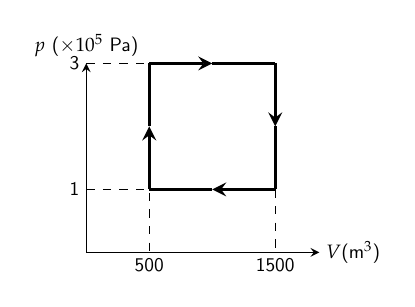
\begin{tikzpicture}[scale=0.8]
\draw[stealth-stealth](0,3)node[above,scale=0.7]{$p$ ($\times 10^5$ Pa)}--(0,0)--(3.7,0)node[right,scale=0.7]{$V$(m$^3$)};
\draw[very thick,-stealth](1,3)--(2,3);
\draw [very thick,-stealth](3,3)--(3,2);
\draw [very thick,-stealth](3,1)--(2,1);
\draw [very thick,-stealth](1,1)--(1,2);
\draw [very thick](2,3)--(3,3)(3,2)--(3,1)(2,1)--(1,1)(1,2)--(1,3);;
\draw[dashed](0,3)--(1,3)(0,1)--(1,1)--(1,0)(3,1)--(3,0);
\node at (0,3) [left,scale=0.7]{3};
\node at (0,1) [left,scale=0.7]{1};
\node at (1,0) [below,scale=0.7]{500};
\node at (3,0) [below, scale =0.7]{1500};
\end{tikzpicture}

Mesin kalor tersebut digunakan untuk menggerakkan sebuah generator yang tegangan keluarnya = 200 V. Jika generator ini mendapat beban arus 5 A mesin kalor tersebut dijalankan pada putaran . . . .
\pilgan {
\item 100 rpm
\item 200 rpm
\item 300 rpm
\item 400 rpm
\item 500 rpm
}

\hide{
}


\end{enumerate}    

\end{multicols*}
 \vspace{1cm}
%-------------------------------------------

 \centering
  \renewcommand{\arraystretch}{2}
  \begin{tabular}{  |>{\centering\arraybackslash}m{4cm}|%
                    >{\centering\arraybackslash}m{11cm}|%
                    >{\centering\arraybackslash}m{4cm}|%
  }
    \hline
    \vspace{0.15cm} 
    \tikz[baseline=(char.base)]{
\draw[green!80!black](-0.3,-0.2) rectangle (0.3,0.2);
\node[green](char){line};
} \small{ arifstwan} &       \textbf{Soal Modul Termodinamika } 
          &  bintangpelajar.com
  \\ \hline 
    
  \end{tabular}
\setlength{\columnsep}{0pt}
\vspace{0.15cm}



\begin{tabular} {|c|c|c|c|c|c|c|c|}
\hline
no & jwb & no & jwb & no & jwb & no & jwb \\ \hline
1 &B  & 11 &A  & 21 &C  & 31&F \\ \hline
2 &D  & 12 &A  & 22 &D  & 32&D  \\ \hline
3 &C  & 13 &B  & 23 &A  & 33&B \\ \hline
4 &D  & 14 &D  & 24 &A  & 34&C \\ \hline
5 &B  & 15 &D  & 25 &E  & 35&B \\ \hline
6 &B  & 16 &C  & 26 &A  & 36&E \\ \hline
7 &E  & 17 &A  & 27 &C  & 37&A \\ \hline
8 &E  & 18 &C  & 28 &E  & 38&A \\ \hline
9 &C  & 19 &B  & 29 &E  & 39&E \\ \hline
10 &B  & 20 & F & 30 & E & 40&D \\ \hline


\end{tabular}

 \end{document}
